%\newcommand{\View}{
%  \href{https://developer.android.com/reference/android/view/View.html}{View}
%}

\newcommand{\Button}{
  \href{https://developer.android.com/reference/android/widget/Button.html}{Button}
}

\newcommand{\Activity}{
  \href{https://developer.android.com/reference/android/app/Activity.html}{Activity}
}

\newcommand{\OnClickListener}{
  \href{https://developer.android.com/reference/android/view/View.OnClickListener.html}{View.OnClickListener}
}

\newcommand{\EditText}{
  \href{https://developer.android.com/reference/android/widget/EditText.html}{EditText}
}

\newcommand{\OnEditorActionListener}{
  \href{https://developer.android.com/reference/android/widget/TextView.OnEditorActionListener.html}{TextView.OnEditorActionListener}
}

\newcommand{\Checkbox}{
  \href{https://developer.android.com/reference/android/widget/CheckBox.html}{Checkbox}
}

\newcommand{\RadioButton}{
  \href{https://developer.android.com/reference/android/widget/RadioButton.html}{RadioButton}
}

\newcommand{\ToggleButton}{
  \href{https://developer.android.com/guide/topics/ui/controls/togglebutton.html}{ToggleButton}
}

\newcommand{\Spinner}{
  \href{https://developer.android.com/reference/android/widget/Spinner.html}{Spinner}
}

\Section{Элементы управления вводом (Input Controls)}

\Subsection{Элементы управления вводом}\\
Элементы управления вводом это интерактивные компоненты в UI приложения.
Андроид предоставляет множество разнообразных контроллеров, которые можно
использовать в UI: кнопки, текстовые поля, флажки, кнопки
масштабирования, кнопки переключения, и много других.

\Subsection{Button, ImageButton}\\
Кнопка, состоящая из текста или иконки (или и того и другого), которые сообщают
какое действие произойдет, когда пользователь коснется кнопки.

XML элемент, который создает кнопку с текстом, используя класс \Button:
\xmlcode{03-input-controls/button.xml}

\Subsubsection{Реагирование на событие нажатия}\\
Когда пользователь нажимает кнопку, объект \Button получает событие нажатия.

Чтобы задать обработчик события нажатия для кнопки, нужно добавить в XML layout
к элементу \textit{<Button>} атрибут \textit{android:onClick}. Значением этого
атрибута должно быть имя метода, который будет вызываться в ответ на событие
нажатия. \Activity, к которой привязан layout, должна затем реализовать
соответствующий метод.

В качестве примера, layout кнопки, использующий \textit{android:onClick}:
\xmlcode{03-input-controls/button_onclick.xml}

Внутри \Activity, к которой привязан этот layout, следующий метод обрабатывает
событие нажатия:
\javacode{03-input-controls/onclick.java}

Метод, объявленный в атрибуте \textit{android:onClick}, должен иметь точно
такую сигнатуру, как показано выше. А именно, метод должен:
\begin{itemize}
  \item Быть \textit{public}.
  
  \item Возвращать \textit{void}
  
  \item Иметь единственный параметр типа \View (это будет \View, который был
  нажат).
\end{itemize}

\Subsubsection{Использование OnClickListener}\\
Также можно объявить обработчик события нажатия программно, а не через XML
layout. Это может быть необходимо, если кнопка создается во время исполнения.

Чтобы объявить обработчик программно, нужно создать объект класса
\OnClickListener и привязать его к кнопке, вызвав
\textit{setOnClickListener(View.OnClickListener)}. Например:
\javacode{03-input-controls/setOnClickListener.java}

Если предыдущий листинг не понятен, то нужно прочитать про анонимные вложенные
классы.

\Subsection{EditText}\\
Текстовое поле позволяет пользователю вводить текст. Поле может быть
однострочным, а может быть многострочным. 

С помощью атрибута \textit{android:inputType} можно указать тип клавиатуры,
которая должна использоваться для объекта \EditText. Например, если нужно,
чтобы пользователь ввел адрес электронной почты, нужно использовать тип
\textit{textEmailAddress}:
\xmlcode{03-input-controls/edit_text.xml}

\Subsubsection{Указание действия на клавиатуре}\\
В дополнении к изменению типа клавиатуры, Андроид позволяет указать действие,
которое нужно сделать, когда пользователь завершил ввод. Выбор действия влияет
на кнопку, которая появится на месте кнопки перевода строки и на действие,
которое нужно выполнить (например, <<Найти>> или <<Отправить>>).

Действие можно указать, задав атрибут \textit{android:imeOptions}. Например,
вот как можно указать действие "Отправить":
\xmlcode{03-input-controls/send_action.xml}

\Subsubsection{Реагирование на событие кнопки}\\
Если через атрибут \textit{android:imeOptions} указано действие
(такое как "actionSend"), то можно слушать различные события, используя 
\OnEditorActionListener. Интерфейс \OnEditorActionListener предоставляет метод
\textit{onEditorAction}, который распознает тип действия с помощью ID дейстивя,
например \textit{IME\_ACTION\_SEND} или \textit{IME\_ACTION\_SEARCH}.

Например, вот как можно слушать событие, которое генерируется, когда
пользователь нажимает на клавиатуре кнопку <<Отправить>>:
\javacode{03-input-controls/onEditorAction.java}

\Subsubsection{AutoCompleteTextView}\\
Для поля ввода можно добавить
\href{https://developer.android.com/guide/topics/ui/controls/text.html#AutoComplete}{автодополнение}.

\Subsection{CheckBox}\\
\Checkbox позволяет пользователю выбрать одну или несколько опция из
набора. Обычно, каждый checkbox следует распологать на отдельной строке.

\image{03-input-controls/checkboxes.png}{Checkbox}

\Subsection{RadioButton}\\
\RadioButton позволяет пользователю выбрать одну опцию из набора. Этот элемент
стоит использовать для взаимоисключающего набора опций, которые должны
отображаться друг за другом.

\image{03-input-controls/radiobuttons.png}{RadioButton}
\pagebreak

\Subsection{ToggleButton}\\
\ToggleButton позволяет пользователю менять опцию между двумя состояниями.

\begin{figure}[H]
\centering
\minipage{0.15\textwidth}
  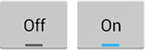
\includegraphics[width=\linewidth]{03-input-controls/togglebutton.png}
  \caption{Toggle buttons}
\endminipage\hspace{1cm}
\minipage{0.2\textwidth}
  
\includegraphics[width=\linewidth]{03-input-controls/switch.png}
  \caption{Switches (начиная с Android 4.0+)}
\endminipage
\end{figure}

\Subsection{Spinner}\\
\Spinner предоставляет быстрый способ выбрать одно значение из набора. По
умолчанию, \Spinner показывает выбранное значение. Касание отображает
выпадающее меню со всеми другими доступными значениями, из которых пользователь
может выбрать новое.

\image{03-input-controls/spinner.png}{Spinner}

\Subsection{DatePickerDialog, TimePickerDialog}\\
Андроид предоставляет
\href{https://developer.android.com/guide/topics/ui/controls/pickers.html}{элементы управления},
которые позволяют пользователю выбрать время или дату.

\image{03-input-controls/pickers.png}{Pickers}
